\section{Split$<$ T $>$ Class Template Reference}
\label{classSplit}\index{Split@{Split}}
A split corresponds to the bipartition of the leaf set induced by an internal edge.  


{\tt \#include $<$extractsplitsforest.h$>$}

Inheritance diagram for Split$<$ T $>$::\begin{figure}[H]
\begin{center}
\leavevmode
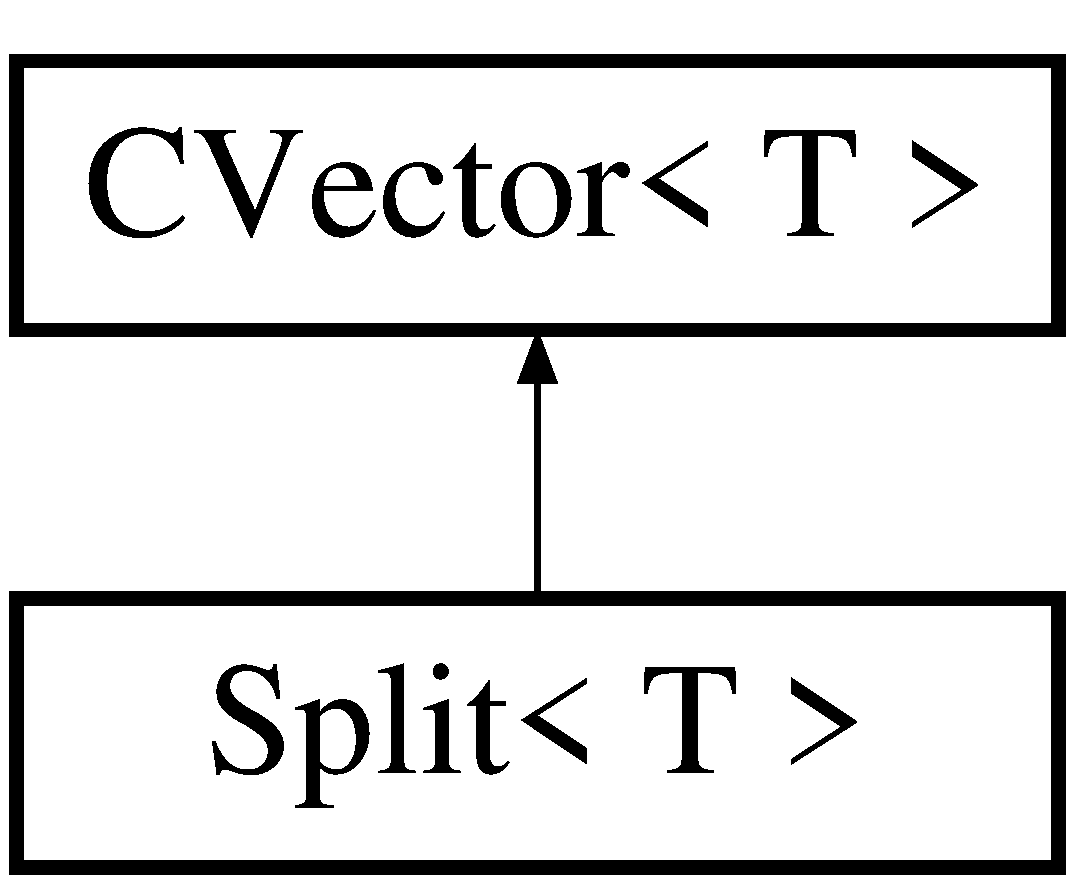
\includegraphics[height=2cm]{classSplit}
\end{center}
\end{figure}
\subsection*{Public Member Functions}
\begin{CompactItemize}
\item 
{\bf Split} ()
\item 
{\bf Split} (size\_\-t)
\item 
bool {\bf operator$<$} (const {\bf Split} \&) const 
\begin{CompactList}\small\item\em whether or not split was flipped \item\end{CompactList}\item 
{\bf Split} ()
\item 
{\bf Split} (size\_\-t)
\item 
bool {\bf operator$<$} (const {\bf Split} \&) const 
\begin{CompactList}\small\item\em starting point of right partition \item\end{CompactList}\end{CompactItemize}
\subsection*{Public Attributes}
\begin{CompactItemize}
\item 
size\_\-t {\bf \_\-rp}
\item 
int {\bf \_\-left}
\begin{CompactList}\small\item\em starting point of right partition \item\end{CompactList}\item 
int {\bf \_\-right}
\begin{CompactList}\small\item\em starting point of right partition \item\end{CompactList}\item 
bool {\bf \_\-flip}
\begin{CompactList}\small\item\em position of split in original tree \item\end{CompactList}\end{CompactItemize}


\subsection{Detailed Description}
\subsubsection*{template$<$class T$>$ class Split$<$ T $>$}

A split corresponds to the bipartition of the leaf set induced by an internal edge. 



\subsection{Constructor \& Destructor Documentation}
\index{Split@{Split}!Split@{Split}}
\index{Split@{Split}!Split@{Split}}
\subsubsection{\setlength{\rightskip}{0pt plus 5cm}template$<$class T$>$ {\bf Split}$<$ T $>$::{\bf Split} ()}\label{classSplit_a0}


\index{Split@{Split}!Split@{Split}}
\index{Split@{Split}!Split@{Split}}
\subsubsection{\setlength{\rightskip}{0pt plus 5cm}template$<$class T$>$ {\bf Split}$<$ T $>$::{\bf Split} (size\_\-t)}\label{classSplit_a1}


\index{Split@{Split}!Split@{Split}}
\index{Split@{Split}!Split@{Split}}
\subsubsection{\setlength{\rightskip}{0pt plus 5cm}template$<$class T$>$ {\bf Split}$<$ T $>$::{\bf Split} ()}\label{classSplit_a3}


\index{Split@{Split}!Split@{Split}}
\index{Split@{Split}!Split@{Split}}
\subsubsection{\setlength{\rightskip}{0pt plus 5cm}template$<$class T$>$ {\bf Split}$<$ T $>$::{\bf Split} (size\_\-t)}\label{classSplit_a4}




\subsection{Member Function Documentation}
\index{Split@{Split}!operator<@{operator$<$}}
\index{operator<@{operator$<$}!Split@{Split}}
\subsubsection{\setlength{\rightskip}{0pt plus 5cm}template$<$class T$>$ bool {\bf Split}$<$ T $>$::operator$<$ (const {\bf Split}$<$ T $>$ \&) const}\label{classSplit_a5}


starting point of right partition 

\index{Split@{Split}!operator<@{operator$<$}}
\index{operator<@{operator$<$}!Split@{Split}}
\subsubsection{\setlength{\rightskip}{0pt plus 5cm}template$<$class T$>$ bool {\bf Split}$<$ T $>$::operator$<$ (const {\bf Split}$<$ T $>$ \&) const}\label{classSplit_a2}


whether or not split was flipped 



\subsection{Member Data Documentation}
\index{Split@{Split}!_flip@{\_\-flip}}
\index{_flip@{\_\-flip}!Split@{Split}}
\subsubsection{\setlength{\rightskip}{0pt plus 5cm}template$<$class T$>$ bool {\bf Split}$<$ T $>$::{\bf \_\-flip}}\label{classSplit_o3}


position of split in original tree 

\index{Split@{Split}!_left@{\_\-left}}
\index{_left@{\_\-left}!Split@{Split}}
\subsubsection{\setlength{\rightskip}{0pt plus 5cm}template$<$class T$>$ int {\bf Split}$<$ T $>$::{\bf \_\-left}}\label{classSplit_o1}


starting point of right partition 

\index{Split@{Split}!_right@{\_\-right}}
\index{_right@{\_\-right}!Split@{Split}}
\subsubsection{\setlength{\rightskip}{0pt plus 5cm}template$<$class T$>$ int {\bf Split}$<$ T $>$::{\bf \_\-right}}\label{classSplit_o2}


starting point of right partition 

\index{Split@{Split}!_rp@{\_\-rp}}
\index{_rp@{\_\-rp}!Split@{Split}}
\subsubsection{\setlength{\rightskip}{0pt plus 5cm}template$<$class T$>$ size\_\-t {\bf Split}$<$ T $>$::{\bf \_\-rp}}\label{classSplit_o0}




The documentation for this class was generated from the following files:\begin{CompactItemize}
\item 
{\bf extractsplitsforest.h}\item 
{\bf splittable.h}\item 
{\bf extractsplitsforest.cpp}\item 
{\bf extractsplitsforest\_\-impl.h}\item 
{\bf splittable\_\-impl.h}\end{CompactItemize}
